\section{Filters}

\begin{figure}
    \centering
    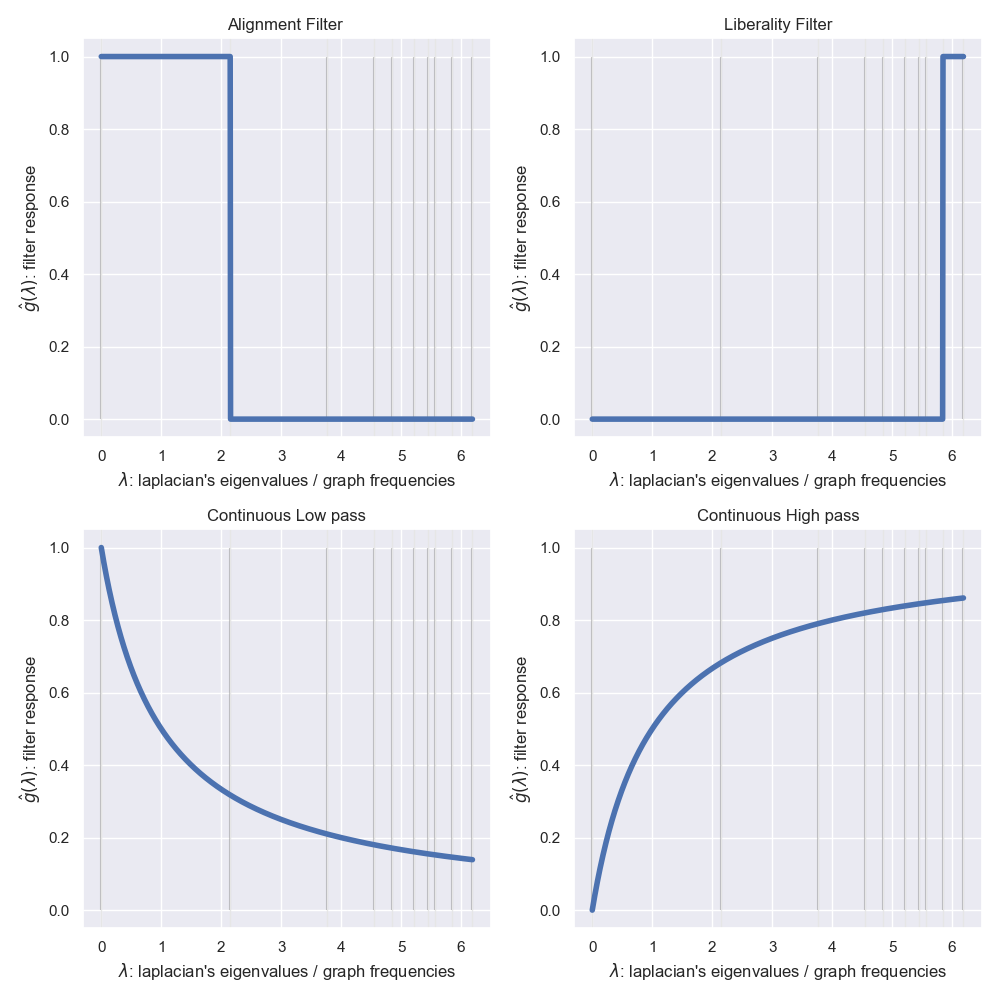
\includegraphics{img/plot_filters.png}
    \caption{Comparison of different filters for graph signal analysis. The \textit{alignment filter} and the \textit{liberality filter} are the low-pass filter and high-pass filter, respectively, employed in the article\cite{huang_graph_2018}. The authors defined their filters by considering the $10$\% lowest and largest eigenvalues, respectively.  In our context, this comes down to filtering approximately 2 eigenvalues.}
    \label{fig:filt}
\end{figure}

\begin{figure}
    \centering
    \begin{subfigure}{\textwidth}
        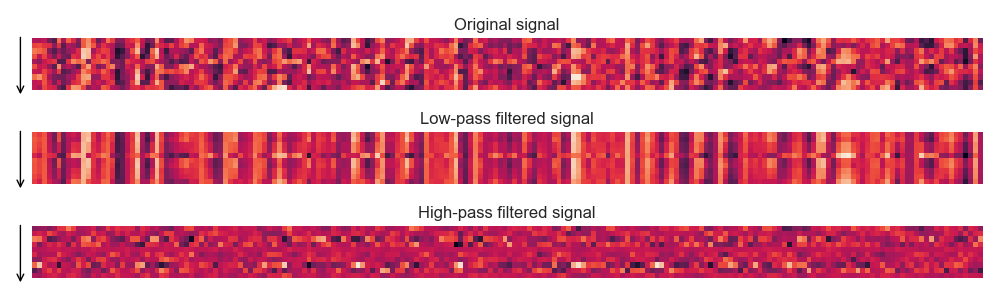
\includegraphics[width=\textwidth]{img/ex_filtered_signal.png}
        \caption{Filtered signal $Y_H$}
    \label{fig/ex_filt_signal}
    \end{subfigure}
    \begin{subfigure}{\textwidth}
        \centering
        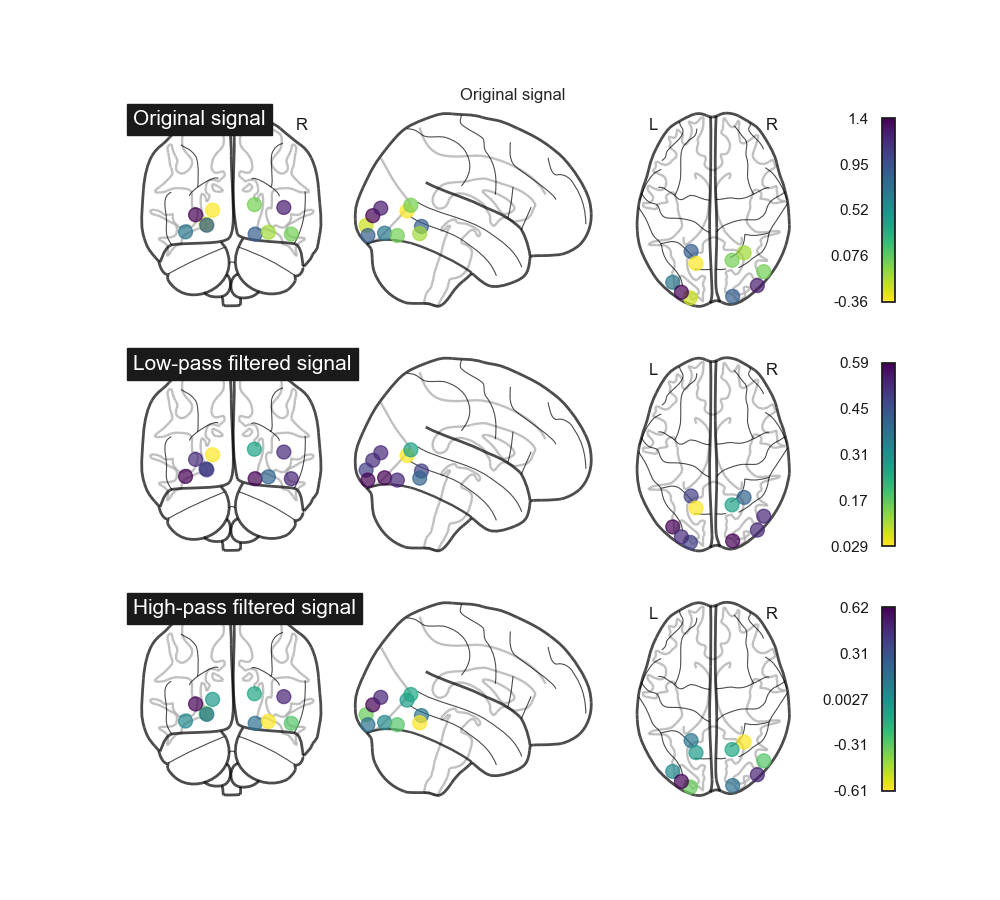
\includegraphics[width=\textwidth]{img/ex_filtered_signal_markers.png}
        \caption{Filtered signal at time $t=0$ in the brain graph.}
        \label{fig:ex_filt_markers}
    \end{subfigure}
    \caption{Visualization of the filtered signals at each time point in (a) and on the graph in (b). (a) The down arrow in $y$-axis indicates the brain regions. The $x$-axis corresponds to the time axis. (b)}
    \label{fig:visu_filt_signal}
\end{figure}

\section{Test statistic}

\begin{figure}
    \centering
    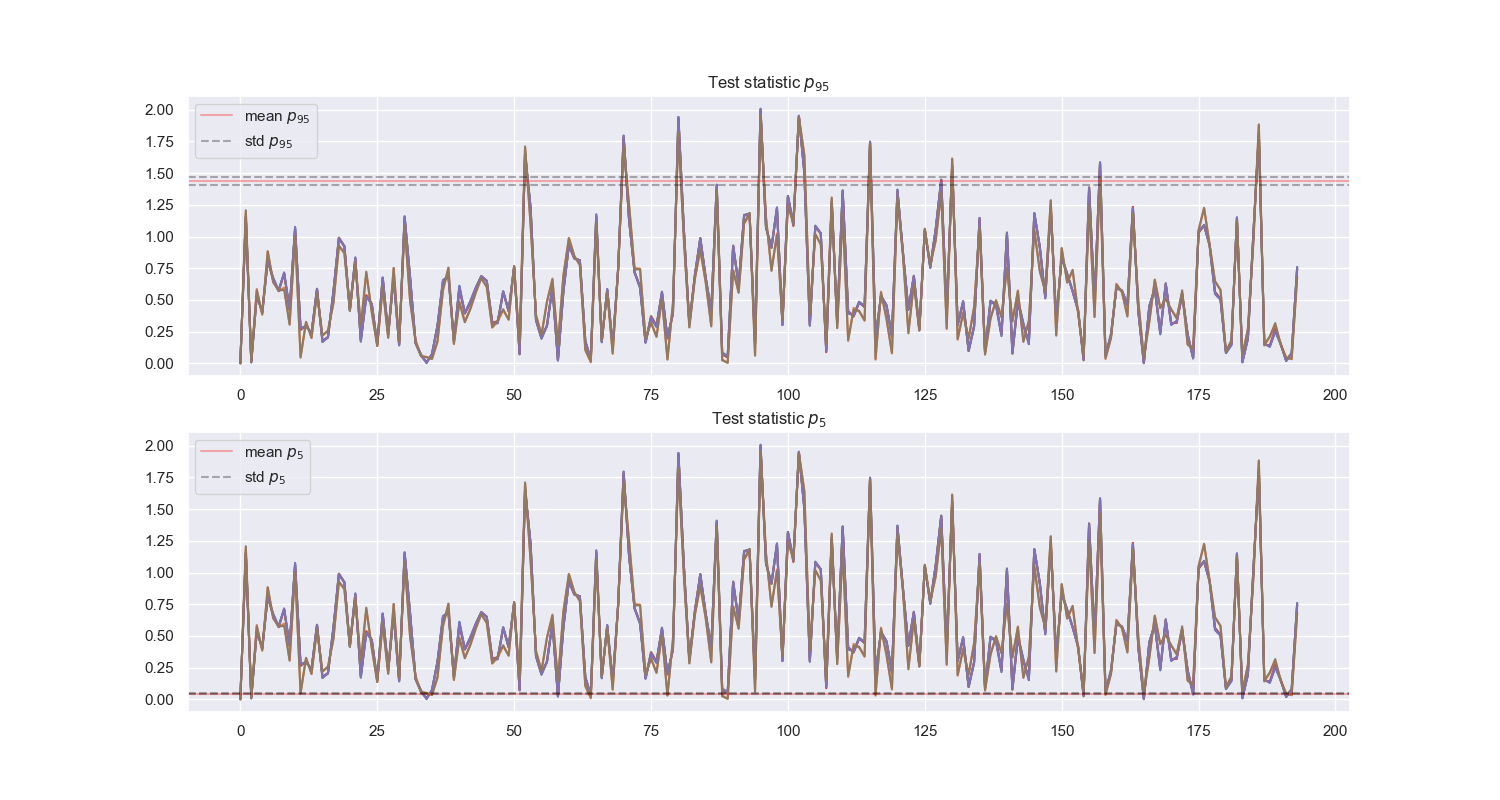
\includegraphics{img/plot_ex_surrogate.png}
    \caption{Threshold computed on the surrogate signals. $p_{95}$ and $p_{5}$ are respectively the average of the 95\% and 5\% (for significant low amplitude) percentile on the surrogate signals.}
    \label{fig:statistic_surr}
\end{figure}

\begin{figure}
    \centering
    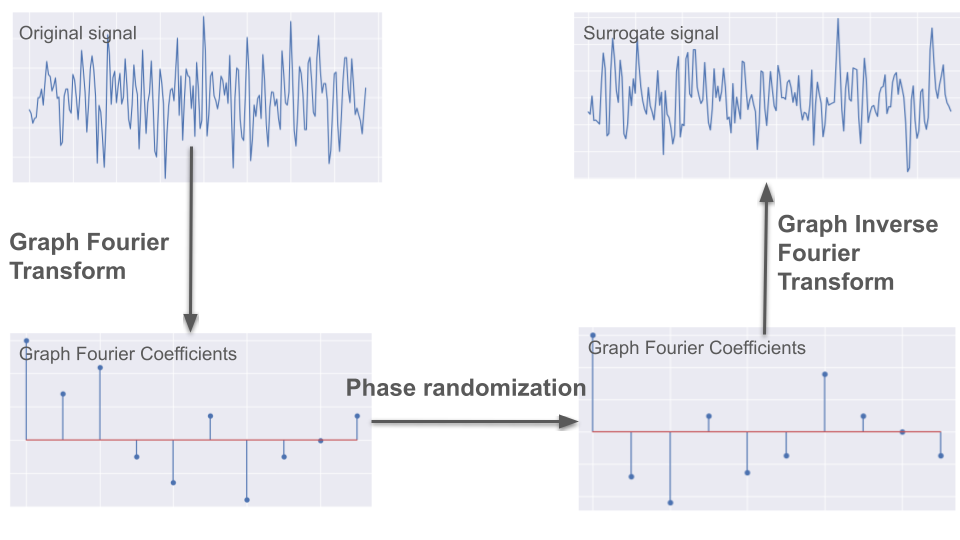
\includegraphics{img/surrogate_scheme.png}
    \caption{Surrogate signal generation scheme.}
    \label{surr_scheme}
\end{figure}

\section{Results on computing excursions}

\begin{figure}
    \centering
    \begin{subfigure}{0.45\textwidth}
        \centering
        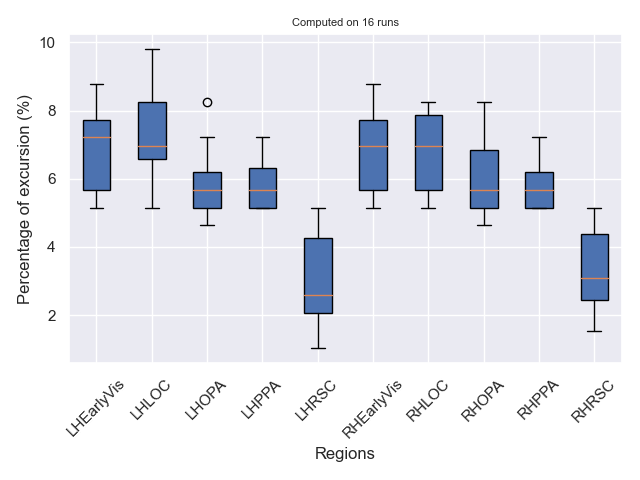
\includegraphics[width=\textwidth]{img/low_non_continuous_filter_graph_randomization.png}
        \caption{Article-inspired low-pass filter}
    \end{subfigure}
    \hfill
    \begin{subfigure}{0.45\textwidth}
        \centering
        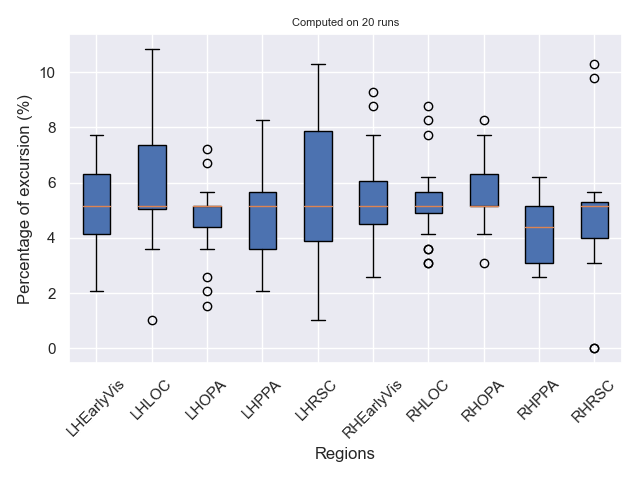
\includegraphics[width=\textwidth]{img/high_non_continuous_filter_graph_randomization.png}
        \caption{Article-inspired high-pass filter}
    \end{subfigure}
    \hfill
    \begin{subfigure}{0.45\textwidth}
        \centering
        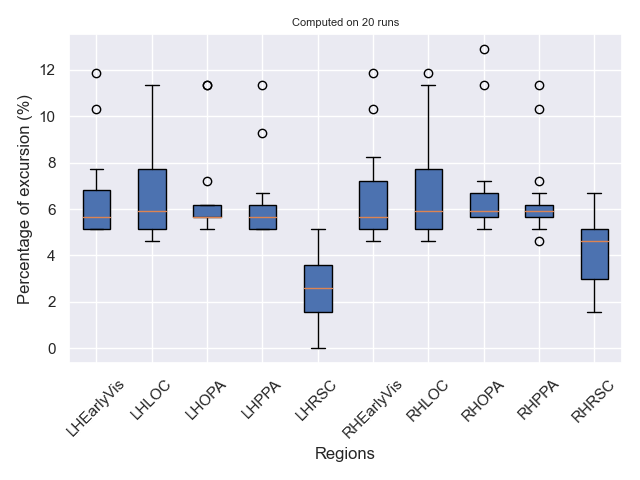
\includegraphics[width=\textwidth]{img/low_continuous_filter_graph_randomization.png}
        \caption{Continuous low-pass filter}
    \end{subfigure}
    \hfill
    \begin{subfigure}{0.45\textwidth}
        \centering
        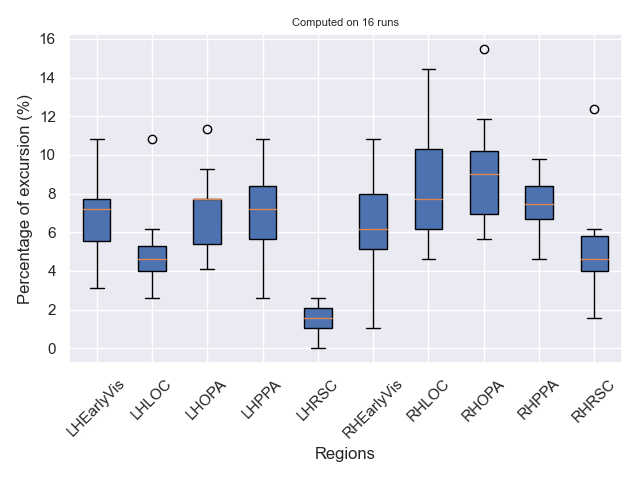
\includegraphics[width=\textwidth]{img/high_continuous_filter_graph_randomization.png}
        \caption{Continuous high-pass filter}
    \end{subfigure}
    \caption{Comparison of different filters for computing excursions in alignment and liberality regimes. The method outlined in section \ref{excursion_results} were repeated on $20$ different fMRI of the same patient. For each run, we generate 1,000 null surrogate graph signal.}
    \label{fig:result_excursions_filters}
\end{figure}

\begin{figure}
    \centering
    \begin{subfigure}{.45\textwidth}
        \centering
        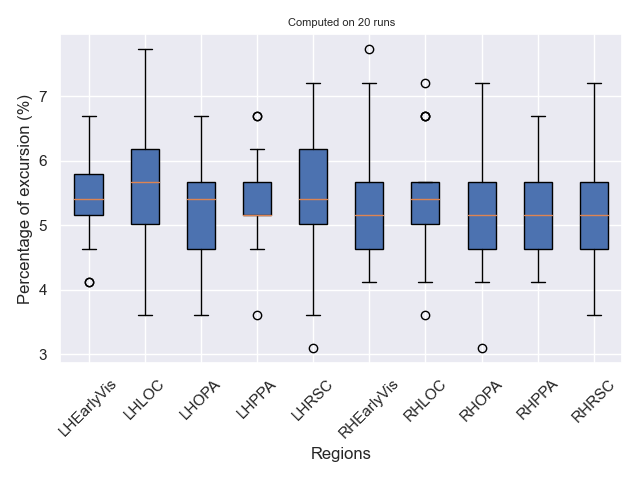
\includegraphics[width=\textwidth]{img/low_continuous_filter_Fourier_randomization.png}
        \caption{Continuous low-pass filter}
    \end{subfigure}
    \hfill
    \begin{subfigure}{.45\textwidth}
        \centering
        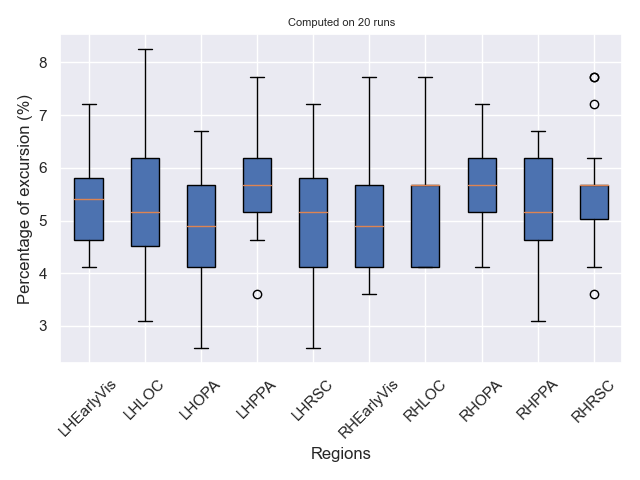
\includegraphics[width=\textwidth]{img/high_continuous_filter_Fourier_randomization.png}
        \caption{Continuous high-pass filter}
    \end{subfigure}
    \caption{Results using the conventional phase Fourier randomization in the temporal domain.}
    \label{fig:result_Fourier_excursions}
\end{figure}